% Front matter: cover page (page 1), contents (page 2+), abstract, notation,
% reproducibility statement.

%---------------------------------------------------------------- cover page
\begin{titlepage}
\centering
\vspace*{1.2cm}
{\Huge\scshape S\,G\,R\ \ A*\par}
\vspace{0.5cm}
{\LARGE A First-Principles Relativistic Simulator of the\\
Galactic-Centre Black Hole\par}
\vspace{0.9cm}
{\large Shadow metrology, S-star orbit fitting, and a free-quadrupole\\
test of the no-hair theorem — with a complete account of the\\
methods, tests, and development of the instrument\par}
\vspace{1.4cm}
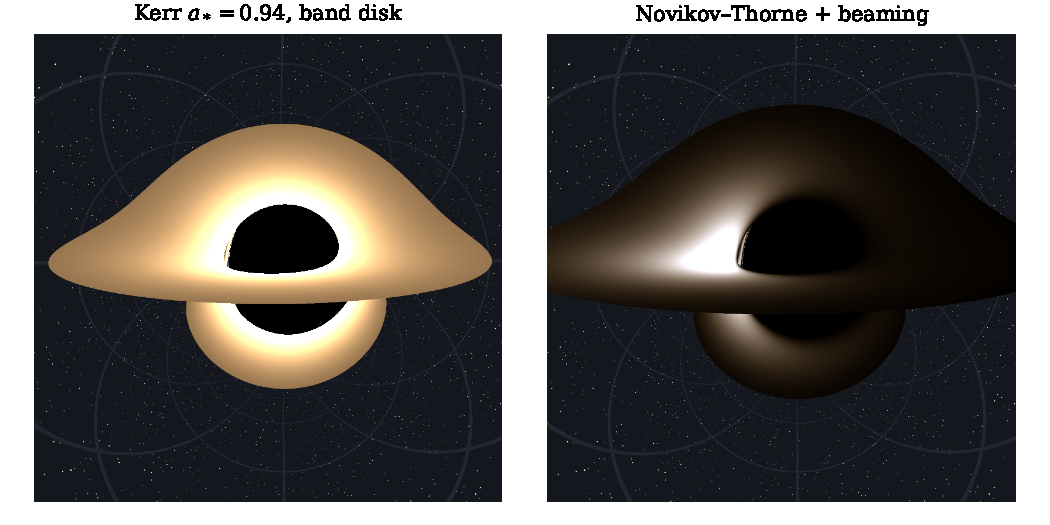
\includegraphics[width=0.82\textwidth]{figures/fig_disk_render.pdf}
\vfill
{\large C.~Excelsis\par}
\vspace{0.3cm}
{\large Independent research report\par}
\vspace{0.3cm}
{\large \today\par}
\end{titlepage}

%---------------------------------------------------------------- contents
\pagenumbering{roman}
\tableofcontents
\listoffigures
\listoftables
\cleardoublepage

%---------------------------------------------------------------- abstract
\chapter*{Abstract}
\addcontentsline{toc}{chapter}{Abstract}

We present a ground-up, physically rigorous simulator of the Galactic-centre
black hole \sgra{}, built on exact Kerr geodesics and validated end-to-end
against published strong-field observations. Null and timelike geodesics are
integrated in a second-order Mino-time formulation of the Carter equations
with per-step constraint projection, conserving $(E, L_z, Q)$ to better than
$10^{-6}$ relative over complete orbits. A CPU reference ray tracer
reproduces the analytic Schwarzschild shadow to a relative accuracy of
$5\times10^{-16}$ and the Bardeen critical curve for spinning holes; a
double-precision GPU compute port agrees with the CPU ground truth to a mean
pixel residual of \GpuMeanDiff. Fitting 13 orbital and potential parameters
to the \FitNAst{} astrometric and \FitNRv{} radial-velocity measurements of
the star S2 \citep{Gillessen2017} with full general-relativistic timelike
geodesics recovers $M = \FitMass \pm \FitMassErr \times 10^{6}\,\msun$ and
$R_0 = \FitDist \pm \FitDistErr$~pc, within $\FitMassNSigma\sigma$ and
$\FitDistNSigma\sigma$ of the GRAVITY interferometric values, at a reduced
$\chi^2$ of \FitChiRed. The model reproduces the gravitational-redshift
excess at the 2018 pericentre passage
($\GrExcessPeak\,\mathrm{km\,s^{-1}}$ peak) detected by
\citet{Gravity2018}, and the Schwarzschild precession of
$\PrecSchw$~arcmin per orbit confirmed by \citet{Gravity2020}. At the
GRAVITY mass and distance the simulated photon ring diameter is
$\CalDiamUas\,\muas$, inside the EHT measurement of
$51.8\pm2.3\,\muas$ \citep{EHT2022}. Freeing the quadrupole moment in a
Hartle--Thorne extension yields
$\epsq = \EpsQBest \pm \EpsQSigma \times 10^{5}$ (68 per cent),
consistent with the no-hair theorem.

This report is the long-form account of that programme. Part~I is a
plain-language primer for readers without a physics background. Parts~II--IV
derive, from first principles, every formula the simulator implements;
document the numerical methods and their error analysis; present the full
results with their statistical treatment; and record the complete
development history, test suite, and validation gates through which the
instrument was built.

% TODO(thesis): expand to ~400 words when the MCMC and cluster-fit results land.

%---------------------------------------------------------------- notation
\chapter*{Notation and Conventions}
\addcontentsline{toc}{chapter}{Notation and Conventions}

Geometric units $G=c=1$ are used throughout unless stated; masses, lengths
and times are quoted in units of the gravitational radius $M$
(for \sgra{}: $GM/c^2 = \UasPerM^{-1}$ scaling on the sky, $GM/c^3 = 21.17$~s).
Metric signature $(-,+,+,+)$; Boyer--Lindquist coordinates
$(t,r,\theta,\phi)$.

% TODO(thesis): full symbol table (M, a, a*, Sigma, Delta, A, E, Lz, Q, mu,
% lambda Mino, tau, eps_q, g, xi, eta, gamma_Lyapunov, chi2, ...).

%------------------------------------------------- reproducibility statement
\chapter*{Reproducibility Statement}
\addcontentsline{toc}{chapter}{Reproducibility Statement}

Every quantitative statement in this report that is not a cited literature
value is typeset from a macro in \texttt{numbers.tex}, generated by
\texttt{scripts/make\_numbers.py} from machine-readable artefacts produced by
the simulation; every figure is generated by \texttt{make figures}
(matplotlib) from the same artefacts. The single command
\texttt{make reproduce} re-runs the full chain — unit tests, reference
renders, sub-ring metrology, orbit fits, calibration, sweeps, and figure
generation — from source. A number that cannot survive this cycle cannot
appear in this document.

\cleardoublepage
\pagenumbering{arabic}
